\iffalse
 

\def\mytitle{MATRICES USING PYTHON}
\def\myauthor{THOUTU RAHUL RAJ}
\def\contact{rdj4648@gmail.com}
\def\mymodule{Future Wireless Communication (FWC)}
\documentclass[10pt, a4paper]{article}
\usepackage[a4paper,outer=1.5cm,inner=1.5cm,top=1.75cm,bottom=1.5cm]{geometry}
\twocolumn
\usepackage{graphicx}
\graphicspath{{./images/}}
\usepackage[colorlinks,linkcolor={black},citecolor={blue!80!black},urlcolor={blue!80!black}]{hyperref}
\usepackage[parfill]{parskip}
\usepackage{lmodern}
\usepackage{amsmath,amsfonts,amssymb,amsthm}
\usepackage{tikz}
	\usepackage{physics}
%\documentclass[tikz, border=2mm]{standalone}
\usepackage{karnaugh-map}
%\documentclass{article}
\usepackage{tabularx}
\usepackage{circuitikz}
\usetikzlibrary{calc}
\usepackage{amsmath}
\usepackage{amssymb}
\renewcommand*\familydefault{\sfdefault}
\usepackage{watermark}
\usepackage{lipsum}
\usepackage{xcolor}
\usepackage{listings}
\usepackage{float}
\usepackage{titlesec}
\providecommand{\norm}[1]{\left\lVert#1\right\rVert}
\providecommand{\sbrak}[1]{\ensuremath{{}\left[#1\right]}}
\providecommand{\lsbrak}[1]{\ensuremath{{}\left[#1\right.}}
\providecommand{\rsbrak}[1]{\ensuremath{{}\left.#1\right]}}
\providecommand{\brak}[1]{\ensuremath{\left(#1\right)}}
\providecommand{\lbrak}[1]{\ensuremath{\left(#1\right.}}
\providecommand{\rbrak}[1]{\ensuremath{\left.#1\right)}}
\providecommand{\cbrak}[1]{\ensuremath{\left\{#1\right\}}}
\providecommand{\lcbrak}[1]{\ensuremath{\left\{#1\right.}}
\providecommand{\rcbrak}[1]{\ensuremath{\left.#1\right\}}}
\newcommand{\myvec}[1]{\ensuremath{\begin{pmatrix}#1\end{pmatrix}}}
\let\vec\mathbf
\providecommand{\mtx}[1]{\mathbf{#1}}
\titlespacing{\subsection}{1pt}{\parskip}{3pt}
\titlespacing{\subsubsection}{0pt}{\parskip}{-\parskip}
\titlespacing{\paragraph}{0pt}{\parskip}{\parskip}
\newcommand{\figuremacro}[5]

\begin{document}

\title{\mytitle}
\author{\myauthor\hspace{1em}\\\contact\\FWC22008\hspace{6.5em}IITH\hspace{0.5em}\mymodule\hspace{6em}ASSIGN-4}
\date{}
	\maketitle
		
	\tableofcontents
\vspace{5mm}
\fi
If diagonals of a parallelogram are equal then show that it is a rectangle.

	\begin{figure}[!h]
		\centering
		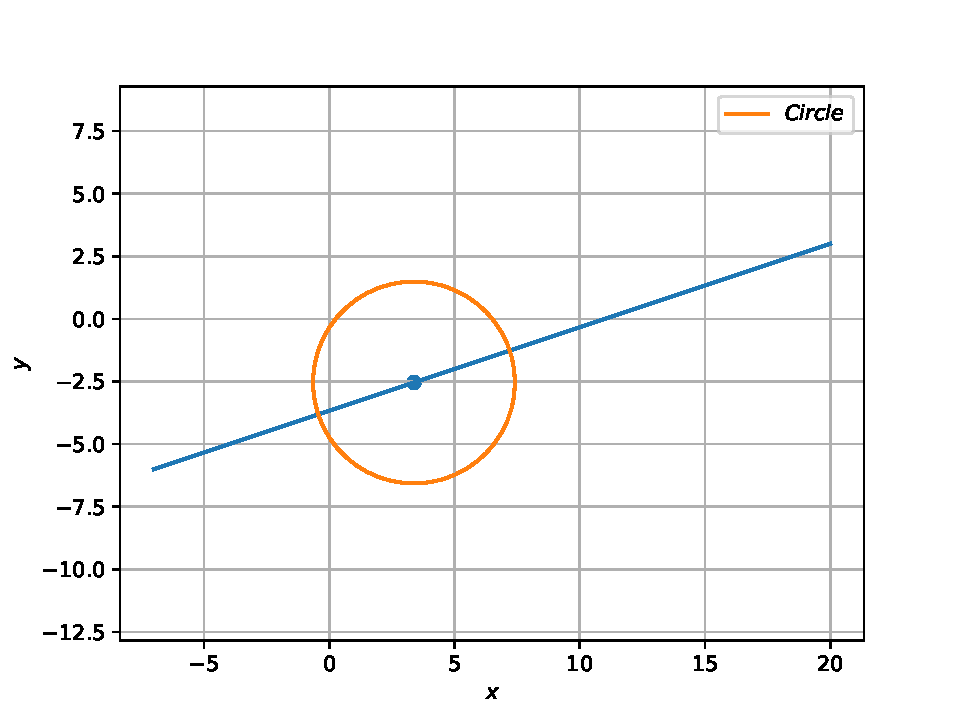
\includegraphics[width=\columnwidth]{chapters/9/8/1/2/fig.pdf}
     %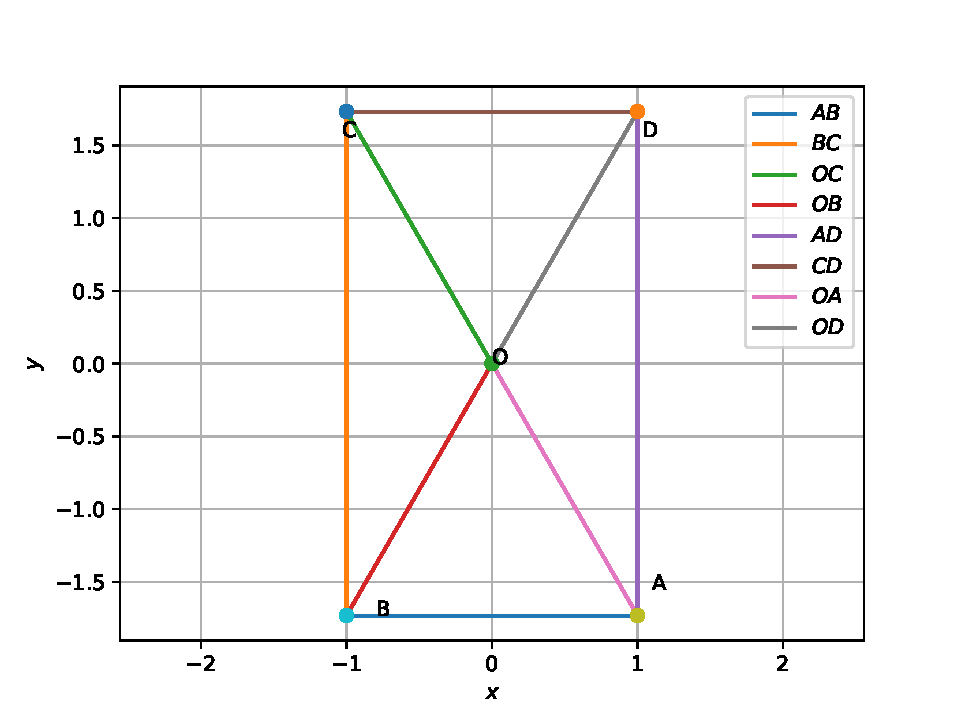
\includegraphics[scale=0.5]{fig.pdf} 
		\caption{}
		\label{fig:9/8/1/2}
  	\end{figure}
	\solution 
   See Fig. 
		\ref{fig:9/8/1/2}.
   From 
	  \eqref{eq:two-pgm}, 
\begin{align}
	  \label{eq:two-pgm-def} 
 \vec{B} - \vec{A}= \vec{C}-\vec{D}
 \\
\implies  \vec{B} - \vec{C}= \vec{A}-\vec{D}
	\end{align}
	Also, it is given that the diagonals of $ABCD$ are equal.  Hence, 
\begin{align}
	\norm{\vec{C} - \vec{A}}^2&= \norm{\vec{D}-\vec{B}}^2
 \\
	\implies 
	\norm{(\vec{C}-\vec{B}) + (\vec{B}-\vec{A})}^2 &= \norm{(\vec{D}-\vec{C}) + (\vec{C}-\vec{B}}^2
\end{align}
which can be expressed as
\begin{multline}
	\norm{\vec{C}-\vec{B}}^2 + \norm{\vec{B}-\vec{A}}^2 + 2(\vec{C}-\vec{B})^{\top} (\vec{B}-\vec{A}) 
	\\
	= \norm{\vec{D}-\vec{C}}^2 + \norm{\vec{C}-\vec{B}}^2+2(\vec{D}-\vec{C})^{\top} (\vec{C}-\vec{B}) 
\end{multline}
which, can be simplified to obtain 
\begin{align}
	(\vec{C}-\vec{B})^{\top} (\vec{B}-\vec{A})&=(\vec{D}-\vec{C})^{\top} (\vec{C}-\vec{B}) 
\end{align}
since 
\begin{align}
\norm{\vec{D}-\vec{C}} =   
\norm{\vec{B}-\vec{A}}   
\end{align}
yielding 
\begin{align}
	(\vec{A}-\vec{B})^{\top} (\vec{B}-\vec{C})=\vec{0}
\end{align}
	  from \eqref{eq:two-pgm-def}.  
